\begin{figure}[H]
  \centering
  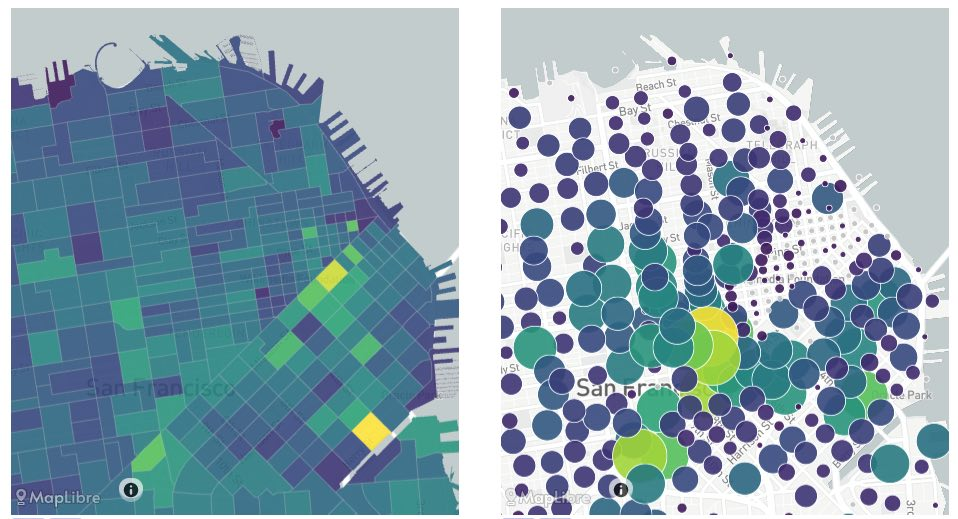
\includegraphics[width=0.8\textwidth]{assets/area-maps.jpg}
  \caption{Area map with color-filled areas; Area map with circles instead of filled areas}
\end{figure}

Area maps with filled colors are excellent for depicting spatial data in
one dimension.

\hypertarget{creating-this-panel}{%
\subsection{Creating this panel}\label{creating-this-panel}}

Properties are written in either a standalone \texttt{viz-map*.yaml}
file, or in a dashboard file they go in the \texttt{layout:} section of
a \texttt{dashboard-*.yaml} file. See the examples at the end of this
document.

\textbf{Standalone:} Create a \texttt{viz-map*.yaml} file as described
below

-or-

\textbf{Embed in Dashboard:} Create a \texttt{dashboard-*.yaml} file and
include a \texttt{type:\ map} section as described below.

\begin{itemize}
\tightlist
\item
  Each area map panel is defined inside a \textbf{row} in a
  \texttt{dashboard-*.yaml} file.
\item
  Use panel \texttt{type:\ map} in the dashboard configuration. (Note
  this may change in the future as we add more map types)
\item
  Standard title, description, and width fields define the frame.
\item
  See \href{dashboards}{Dashboard documentation} for general tips on
  creating dashboard configurations.
\end{itemize}

\hypertarget{properties}{%
\subsection{Properties}\label{properties}}

\hypertarget{dashboard-specific-properties}{%
\subsubsection{Dashboard-specific
properties}\label{dashboard-specific-properties}}

\begin{longtable}[]{@{}
  >{\raggedright\arraybackslash}p{(\columnwidth - 2\tabcolsep) * \real{0.5000}}
  >{\raggedright\arraybackslash}p{(\columnwidth - 2\tabcolsep) * \real{0.5000}}@{}}
\toprule()
\begin{minipage}[b]{\linewidth}\raggedright
Property
\end{minipage} & \begin{minipage}[b]{\linewidth}\raggedright
Usage
\end{minipage} \\
\midrule()
\endhead
\texttt{type} & In \texttt{dashboard-*.yaml} config files, MUST be set
to \textbf{``map''} \\
\texttt{height} & Relative height. Larger numbers create taller panels.
(default: 5) \\
\texttt{width} & Relative width. The widths of all panels on a single
row are summed, and the layout of each panel is then relative to that
total width. (default: 1) \\
\bottomrule()
\end{longtable}

\hypertarget{general-properties}{%
\subsubsection{General properties}\label{general-properties}}

\begin{longtable}[]{@{}
  >{\raggedright\arraybackslash}p{(\columnwidth - 2\tabcolsep) * \real{0.5000}}
  >{\raggedright\arraybackslash}p{(\columnwidth - 2\tabcolsep) * \real{0.5000}}@{}}
\toprule()
\begin{minipage}[b]{\linewidth}\raggedright
Property
\end{minipage} & \begin{minipage}[b]{\linewidth}\raggedright
Usage
\end{minipage} \\
\midrule()
\endhead
\texttt{title}, \texttt{title\_en}, \texttt{title\_de} & Title text for
this panel; will be shown just above the map. The language-specific
version will be used if provided. \\
\texttt{description}, \texttt{description\_en}, \texttt{description\_de}
& Second line of descriptive text, shown below the title line. The
language-specific version will be used if provided. \\
\texttt{center} & Coordinates that the map centers on. Can be provided
as array or string. If it is not provided, a center is calculated using
a sampling of the data. \\
\texttt{zoom} & Zoom level of the map between 5 and 20. (default: 9) \\
\texttt{pitch} & Map pitch (default: 0) \\
\texttt{bearing} & Map bearing/direction (default:0) \\
\bottomrule()
\end{longtable}

\hypertarget{shapes-the-boundariesareas-to-be-drawn}{%
\subsubsection{\texorpdfstring{\textbf{shapes:} the boundaries/areas to
be
drawn}{shapes: the boundaries/areas to be drawn}}\label{shapes-the-boundariesareas-to-be-drawn}}

There are \textbf{two separate data types} required for an area map: the
boundaries/shapes, and one the dataset (unless the shapefile
self-contains all of the required data).

Both files must contain an matching identification column in order to
\textbf{join the two datasets} together. In other words, the boundary
IDs must be present (somewhere) in both datafiles. The names of the
columns do not have to be identical, but it helps legibility. See below.

\begin{lstlisting}
shapes:
  file: my-taz-shapefile.shp
  join: id
\end{lstlisting}

Contains two subentries:

\begin{itemize}
\tightlist
\item
  \textbf{file:} String. The filepath containing the data. May include
  wildcards * and ?. File can be in \emph{geojson} format, or a
  \emph{shapefile}. File type is determined by suffix, so must end in
  either \texttt{.geojson} or \texttt{.shp} When loading shapefiles, an
  identically-named .dbf and .prj file will also be read from the same
  folder. Be sure to supply a .prj file containing a valid EPSG code if
  your data is not in lat/long format.
\item
  \textbf{join:} String. The name of the data column containing shape
  IDs, or `id' if it is in the id field of geojson.
\end{itemize}

\hypertarget{datasets-the-dataset-to-be-joined-to-the-shapefile}{%
\subsubsection{\texorpdfstring{\textbf{datasets:} the dataset to be
joined to the
shapefile}{datasets: the dataset to be joined to the shapefile}}\label{datasets-the-dataset-to-be-joined-to-the-shapefile}}

\begin{lstlisting}
  datasets:
    transit-trips:
      file: .summaries/transit-outputs.csv
      join: TAZ
\end{lstlisting}

Contains an object naming the dataset and providing its filename and
join column:

\begin{itemize}
\tightlist
\item
  \textbf{name of dataset:} Give the dataset a simple name, which will
  be used in the display settings below. e.g.~\texttt{tazdata}

  \begin{itemize}
  \tightlist
  \item
    \textbf{file:} String. The filepath containing the data. May include
    wildcards * and ?. File can be in \emph{CSV or DBF} format. Any
    filename not ending in \texttt{.dbf} will be parsed as a CSV file,
    using either commas, tabs, or spaces as delimiters.
  \item
    \textbf{join:} String. The name of the data column containing the
    shape IDs for joining.
  \end{itemize}
\end{itemize}

\hypertarget{display-define-the-color-and-value-details}{%
\subsubsection{\texorpdfstring{\textbf{display:} define the color and
value
details}{display: define the color and value details}}\label{display-define-the-color-and-value-details}}

For area maps, the \texttt{fill} section defines the color fill, and is
(currently) the only section that is required. At a later date we may
include borders, etc.

\begin{lstlisting}
display:
  fill:
    dataset: transit-trips
    join: TAZ
    filters: operator, income
    columnName: trip_origins, trip_boards, trip_reslocs
    colorRamp:
      ramp: Plasma
      reversed: true
      steps: 5
\end{lstlisting}

\textbf{dataset:} Name of the dataset from above which includes the
data.

\textbf{filters:} (optional) List of any columns which can be used as
category filters by the user interactively. Note that \emph{active
filters} will be shown in the URL bar, so curated maps can be shared via
URL.

\textbf{columnName:} The column name (or names) containing values to be
plotted. If multiple rows have a matching shape ID, all values will be
summed together. (Other stats to be added)

\textbf{colorRamp:} Describe the colors themselves:

\begin{itemize}
\tightlist
\item
  \textbf{ramp:} Name of the color ramp to use.

  \begin{itemize}
  \tightlist
  \item
    Sequential: \texttt{Viridis} \texttt{Plasma} \texttt{Blues}
    \texttt{Greens} \texttt{Purples} \texttt{Oranges}
  \item
    Diverging: \texttt{PRGn} \texttt{RdBu}
  \item
    Categorical: \texttt{Tableau10} \texttt{Paired}. Note categoricals
    only have ten or twelve categories.
  \end{itemize}
\item
  \textbf{reversed:} true/false
\item
  \textbf{steps:} Number of steps in the ramp.
\item
  \textbf{exponentColors:} Optional true/false. If true, values will be
  scaled exponentially before being drawn. This is often useful if
  values are concentrated in small areas, and much higher in value than
  in typical areas.
\item
  \textbf{diff:} Example \texttt{col1\ -\ col2} will activate diff mode

  \begin{itemize}
  \tightlist
  \item
    \emph{(todo: more examples needed )}
  \end{itemize}
\end{itemize}

\hypertarget{filters}{%
\subsubsection{filters}\label{filters}}

In the \texttt{filter} section, you can filter dataset with multiple
expressions on numerical columns in any dataset. Keys are of the format
\texttt{dataset.column:\ "filter"} and filter can be
\texttt{==,\ !=,\ \textless{},\ \textless{}=,\ \textgreater{},\ \textgreater{}=}

\begin{lstlisting}
filters:
  dataset1.trips: "> 0"
  shapes.TAZ: "!=0"

\end{lstlisting}

\hypertarget{tooltip}{%
\subsubsection{Tooltip}\label{tooltip}}

By default, the tooltip shows all columns in the shapefile, as well as
any columns that are actively being displayed as either a color or a
width.

You can customize the tooltip to just show what you are interested as
follows:

\begin{itemize}
\tightlist
\item
  Add a \texttt{tooltip:} section to the properties, which will be an
  array of tooltip entries
\item
  Each entry is of format \texttt{datasetname:columnname}, so for
  example \texttt{AM\_FLOWS:VEHICLE\_VOL} will display the AM\_FLOWS
  dataset and VEHICLE\_VOL column.
\item
  Use the shapefile/network filename for its columnar data, or the
  dataset ``key'' for joined datasets.
\end{itemize}

\textbf{Custom tooltip example:}

\begin{lstlisting}
tooltip:
  - AM:TOT_VOL
  - AM:TNC
  - freeflow.shp:FACILITY_TYPE
  - freeflow.shp:SPEED
\end{lstlisting}

\hypertarget{visualization-hints}{%
\subsection{Visualization hints}\label{visualization-hints}}

Very large and very small areas on the same maps can create misleading
visualizations; consider ``normalizing'' data by land area before
plotting it. Alternatively, the circle-plots show exactly the same data
in a different manner.

\begin{itemize}
\tightlist
\item
  Use the sequential color palettes for continuous data.
\item
  Use diverging color palettes for difference plots and other situations
  where data is both positive and negative
\item
  Use categorical colors when there are just a few categories or
  ``buckets'' in which the data resides.
\end{itemize}

\hypertarget{example-yaml-configurations-putting-it-all-together}{%
\subsection{Example YAML configurations: putting it all
together}\label{example-yaml-configurations-putting-it-all-together}}

\hypertarget{sample-viz-map-1.yaml-standalone-configuration}{%
\subsubsection{Sample viz-map-1.yaml standalone
configuration}\label{sample-viz-map-1.yaml-standalone-configuration}}

\begin{lstlisting}
  title: 'VIZ-MAP 1'
  description: 'All day transit usage'
  center: [6.9814, 51.57]
  zoom: 10
  shapes:
    file: '../../shapefiles/geoid.geojson'
    join: id
  datasets:
    transit-trips:
      file: .dashboard/transit-data.csv
  display:
    fill:
      dataset: transit-trips
      join: geoid
      filters: operator, income
      columnName: trip_origins, trip_boards, trip_reslocs
      colorRamp:
        ramp: Plasma
        steps: 7
\end{lstlisting}

